

\documentclass{article}

\usepackage[top=3cm, bottom=3cm, outer=3cm, inner=3cm]{geometry}
\usepackage{multicol}
\usepackage{graphicx}
\usepackage{url}
\usepackage{hyperref}
\usepackage{array}
\usepackage{natbib}
\usepackage{pdfpages}
\usepackage{multirow}
\usepackage[normalem]{ulem}
\useunder{\uline}{\ul}{}
\usepackage{svg}
\usepackage{xcolor}
\usepackage{listings}
\usepackage{caption}
\usepackage{subcaption}
\usepackage{float}
\usepackage{colortbl}
\usepackage{color}


\newcolumntype{x}[1]{>{\centering\arraybackslash\hspace{0pt}}p{#1}}
\newcolumntype{M}[1]{>{\centering\arraybackslash}m{#1}}
\newcolumntype{N}{@{}m{0pt}@{}}



\newcommand{\itemEmail}{}
\newcommand{\itemStudent}{Edu Breyner Mio Alviz }
\newcommand{\itemCourse}{Introducción al Desarrollo Web}
\newcommand{\itemCourseCode}{20251174}
\newcommand{\itemSemester}{II}
\newcommand{\itemUniversity}{Universidad Nacional de San Agustín de Arequipa}
\newcommand{\itemFaculty}{Facultad de Ingeniería de Producción y Servicios}
\newcommand{\itemDepartment}{Departamento Académico de Ingeniería de Sistemas e Informática}
\newcommand{\itemSchool}{Escuela Profesional de Ingeniería de Sistemas}
\newcommand{\itemAcademic}{2026 - B}
\newcommand{\itemInput}{1 de setiembre}
\newcommand{\itemOutput}{7 de setiembre}
\newcommand{\itemPracticeNumber}{01}
\newcommand{\itemTheme}{Entorno Web, HTTP y HTML Semántico}



\usepackage[english,spanish]{babel}
\usepackage[utf8]{inputenc}

\AtBeginDocument{\selectlanguage{Spanish}}

\renewcommand{\figurename}{Figura}
\renewcommand{\refname}{Referencias}
\renewcommand{\tablename}{Tabla}

\AtBeginDocument{
    \renewcommand\tablename{Tabla}
}


\usepackage{fancyhdr}

\pagestyle{fancy}
\fancyhf{}

\setlength{\headheight}{40.51407pt}

\renewcommand{\headrulewidth}{1pt}
\renewcommand{\footrulewidth}{1pt}


 \fancyhead[L]{\raisebox{-0.2\height}{
\includegraphics[width=3cm]{img/logo_episunsa.png}}}

\fancyhead[C]{
    \fontsize{7}{7}\selectfont
    \itemUniversity \\
    \itemFaculty \\
    \itemDepartment \\
    \itemSchool \\
    \textbf{\itemCourse}
}

 \fancyhead[R]{\raisebox{-0.2\height}{
\includegraphics[width=1.2cm]{img/logo_abet.png}}}

\fancyfoot[L]{Estudiante \itemStudent}
\fancyfoot[C]{\itemCourse}
\fancyfoot[R]{Página \thepage}



\definecolor{dkgreen}{rgb}{0,0.6,0}
\definecolor{gray}{rgb}{0.5,0.5,0.5}
\definecolor{mauve}{rgb}{0.58,0,0.82}
\definecolor{codebackground}{rgb}{0.95,0.95,0.92}
\definecolor{tablebackground}{rgb}{0.8,0,0}

\lstset{
    frame=tb,
    language=html,
    aboveskip=3mm,
    belowskip=3mm,
    showstringspaces=false,
    columns=flexible,
    basicstyle={\small\ttfamily},
    numbers=left,
    numberstyle=\tiny\color{gray},
    keywordstyle=\color{blue},
    commentstyle=\color{dkgreen},
    stringstyle=\color{mauve},
    breaklines=true,
    breakatwhitespace=true,
    tabsize=3,
    backgroundcolor=\color{codebackground}
}


\begin{document}

\vspace*{10px}


\begin{center}
    \fontsize{17}{17}
    \textbf{Informe de Laboratorio \itemPracticeNumber}
\end{center}

\centerline{\textbf{\Large Tema: \itemTheme}}

\vspace{0.3cm}


\begin{flushright}
    \begin{tabular}{|M{2.5cm}|N|}
        \hline
        \rowcolor{tablebackground}
        \color{white}\textbf{Nota} \\
        \hline
        \\[30pt]
        \hline
    \end{tabular}
\end{flushright}


\begin{table}[h!]
    \begin{tabular}{|x{4.7cm}|x{4.8cm}|x{4.8cm}|}
        \hline
        \rowcolor{tablebackground}
        \color{white}\textbf{Estudiante}
        &
        \color{white}\textbf{Escuela}
        &
        \color{white}\textbf{Asignatura}
        \\
        \hline

        {\itemStudent \par \itemEmail}
        &
        \itemSchool
        &
        {\itemCourse \par Semestre: \itemSemester \par Código: \itemCourseCode}

        \\
        \hline
    \end{tabular}
\end{table}


\begin{table}[H]
    \begin{tabular}{|x{4.7cm}|x{4.8cm}|x{4.8cm}|}
        \hline
        \rowcolor{tablebackground}
        \color{white}\textbf{Laboratorio}
        &
        \color{white}\textbf{Tema}
        &
        \color{white}\textbf{Duración}
        \\
        \hline

        \itemPracticeNumber
        &
        \itemTheme
        &
        04 horas

        \\
        \hline
    \end{tabular}
\end{table}



\begin{table}[H]
    \begin{tabular}{|x{4.7cm}|x{4.8cm}|x{4.8cm}|}
        \hline
        \rowcolor{tablebackground}
        \color{white}\textbf{Semestre académico}
        &
        \color{white}\textbf{Fecha de inicio}
        &
        \color{white}\textbf{Fecha de entrega}
        \\
        \hline

        \itemAcademic
        &
        \itemInput
        &
        \itemOutput

        \\
        \hline
    \end{tabular}
\end{table}


\section{Tarea}

La tarea del Laboratorio 01 consiste en configurar el entorno de
desarrollo web y aplicar conceptos básicos de HTTP y HTML5 semántico.

Las actividades realizadas fueron:

\begin{itemize}

    \item Configurar el entorno de desarrollo para trabajar con
    tecnologías web.

    \item Comprender el funcionamiento básico del protocolo HTTP.

    \item Utilizar las herramientas de desarrollador del navegador
    para observar solicitudes y respuestas HTTP.

    \item Crear una página web utilizando HTML5 semántico.

    \item Utilizar elementos como
    \texttt{header}, \texttt{nav}, \texttt{main},
    \texttt{section}, \texttt{article} y \texttt{footer}.

    \item Incorporar elementos multimedia y contenido accesible.

    \item Crear una tabla utilizando \texttt{thead} y \texttt{tbody}.

    \item Crear un formulario de contacto.

    \item Organizar el proyecto utilizando GitHub.

    \item Registrar los avances mediante commits descriptivos.

\end{itemize}


\section{Equipos, materiales y temas utilizados}

\begin{itemize}

    \item Computadora o laptop.

    \item Sistema operativo Windows o GNU/Linux.

    \item Navegador web Google Chrome o Mozilla Firefox.

    \item Visual Studio Code.

    \item Git.

    \item GitHub.

    \item HTML5.

    \item CSS3.

    \item Herramientas de desarrollador del navegador.

    \item Protocolo HTTP.

    \item HTML semántico.

    \item Accesibilidad web.

\end{itemize}


\section{URL de Repositorio GitHub}

\begin{itemize}

    \item URL del repositorio principal:

    \url{https://github.com/emioa-bit/idweb}

    \item URL correspondiente al Laboratorio 01:

    \url{https://github.com/emioa-bit/idweb/tree/main/Lab01}

\end{itemize}


\section{Actividades con el repositorio GitHub}

\subsection{Creación del repositorio}

Se creó un repositorio público denominado
\textbf{IDWeb} para almacenar los trabajos correspondientes
al curso de Introducción al Desarrollo Web.

El repositorio contiene una carpeta denominada
\textbf{Lab01}, donde se almacenan los archivos correspondientes
al primer laboratorio.

\subsection{Estructura del laboratorio}

La estructura desarrollada para el Laboratorio 01 es la siguiente:

\begin{lstlisting}[language=bash]
IDWeb/
|--- Lab01/
|   |--- index.html
|   |--- author.html
|   |--- system.html
|   |--- w3c.html
|   |--- contact.html
|   |
|   |--- css/
|   |   |--- style.css
|   |
|   |--- img/
|       |--- photo.png
\end{lstlisting}

Esta estructura permite mantener separados los documentos HTML,
las hojas de estilos CSS y los recursos gráficos utilizados
en el proyecto.

\subsection{Página principal}

Se creó el archivo \textbf{index.html}, que funciona como página
principal del portafolio académico.

La página utiliza una estructura HTML5 semántica:

\begin{lstlisting}[language=HTML]
<header>
    <h1>Mi Portafolio Académico</h1>

    <nav>
        <ul>
            <li><a href="author.html">Autor</a></li>
            <li><a href="system.html">
                Ingeniería de Sistemas
            </a></li>
            <li><a href="w3c.html">W3C</a></li>
            <li><a href="contact.html">Contacto</a></li>
        </ul>
    </nav>
</header>

<main>
    <section>
        <h2>Bienvenido</h2>
        <p>
            Este es mi portafolio académico del curso
            Introducción al Desarrollo Web.
        </p>
    </section>
</main>

<footer>
    <p>© 2026 - Mi Portafolio Académico</p>
</footer>
\end{lstlisting}

El elemento \texttt{header} contiene el encabezado y el menú de
navegación, mientras que \texttt{main} contiene el contenido
principal de la página.

\subsection{HTML semántico}

Se utilizaron elementos semánticos de HTML5 para representar
correctamente la estructura del contenido.

Entre los elementos utilizados se encuentran:

\begin{itemize}

    \item \texttt{header}: representa el encabezado.

    \item \texttt{nav}: contiene los enlaces de navegación.

    \item \texttt{main}: contiene el contenido principal.

    \item \texttt{section}: permite organizar el contenido
    en diferentes secciones.

    \item \texttt{article}: representa contenido independiente.

    \item \texttt{figure}: permite representar contenido
    multimedia.

    \item \texttt{figcaption}: proporciona una descripción
    para una figura.

    \item \texttt{footer}: representa el pie de página.

\end{itemize}

El uso de HTML semántico facilita la comprensión del documento
por parte de los navegadores, motores de búsqueda y tecnologías
de asistencia.

\subsection{Imagen y accesibilidad}

Se incorporó una imagen dentro del elemento
\texttt{figure}.

\begin{lstlisting}[language=HTML]
<figure>
    <img src="img/photo.png"
         alt="Foto del autor del portafolio"
         width="200">

    <figcaption>
        Foto del autor
    </figcaption>
</figure>
\end{lstlisting}

El atributo \texttt{alt} proporciona una descripción textual
de la imagen, lo cual mejora la accesibilidad del contenido.


\subsection{Tabla de proyectos}

Se implementó una tabla para mostrar los proyectos académicos.

\begin{lstlisting}[language=HTML]
<table>
    <caption>Proyectos académicos</caption>

    <thead>
        <tr>
            <th scope="col">Proyecto</th>
            <th scope="col">Tecnología</th>
            <th scope="col">Descripción</th>
        </tr>
    </thead>

    <tbody>
        <tr>
            <td>Portafolio web</td>
            <td>HTML y CSS</td>
            <td>Página web académica.</td>
        </tr>
    </tbody>
</table>
\end{lstlisting}

Se utilizaron \texttt{thead} y \texttt{tbody} para organizar
correctamente la información de la tabla.

El atributo \texttt{scope="col"} permite identificar las
columnas de la tabla y mejora su accesibilidad.

\subsection{Formulario de contacto}

Se creó una página denominada \textbf{contact.html}, que contiene
un formulario de contacto.

\begin{lstlisting}[language=HTML]
<form>

    <label for="nombre">Nombre:</label>
    <input type="text"
           id="nombre"
           name="nombre"
           required>

    <label for="correo">
        Correo electrónico:
    </label>

    <input type="email"
           id="correo"
           name="correo"
           required>

    <label for="mensaje">Mensaje:</label>

    <textarea id="mensaje"
              name="mensaje"
              rows="6"
              required>
    </textarea>

    <button type="submit">
        Enviar
    </button>

</form>
\end{lstlisting}

Los elementos \texttt{label} están asociados mediante el atributo
\texttt{for} con los respectivos controles del formulario.

\subsection{Hoja de estilos CSS}

Se creó el archivo:

\begin{lstlisting}[language=bash]
Lab01/css/style.css
\end{lstlisting}

La hoja de estilos permite modificar la presentación visual
de las páginas HTML.

El archivo CSS es enlazado mediante:

\begin{lstlisting}[language=HTML]
<link rel="stylesheet" href="css/style.css">
\end{lstlisting}

De esta manera se separa la estructura HTML de la presentación
visual del sitio web.


\section{HTTP y herramientas de desarrollador}

Se utilizaron las herramientas de desarrollador del navegador
para observar las solicitudes realizadas por la página web.

En la pestaña \textbf{Network} se pueden observar diferentes
solicitudes HTTP realizadas por el navegador.

Entre los códigos de estado estudiados se encuentran:

\begin{itemize}

    \item \textbf{200 OK}: indica que la solicitud fue procesada
    correctamente.

    \item \textbf{301 Moved Permanently}: indica que el recurso
    fue trasladado permanentemente a otra ubicación.

    \item \textbf{404 Not Found}: indica que el recurso solicitado
    no fue encontrado.

    \item \textbf{500 Internal Server Error}: indica que ocurrió
    un error interno en el servidor.

\end{itemize}

\subsection{Código de estado HTTP 200}

Cuando una página o recurso se carga correctamente, el servidor
puede responder con el código:

\begin{lstlisting}[language=bash]
200 OK
\end{lstlisting}

Este código indica que la solicitud fue procesada correctamente.

\subsection{Código de estado HTTP 404}

El código:

\begin{lstlisting}[language=bash]
404 Not Found
\end{lstlisting}

se produce cuando el recurso solicitado no existe o no puede
ser encontrado por el servidor.



\section{Control de versiones con Git y GitHub}

Git se utilizó para registrar los cambios realizados durante
el desarrollo del laboratorio.

GitHub permite almacenar el repositorio de manera remota y
facilita la revisión del trabajo.

Los principales comandos relacionados con Git son:

\begin{lstlisting}[language=bash]
git status
git add .
git commit -m "mensaje del commit"
git push origin main
git log --oneline
\end{lstlisting}


\subsection{Commits realizados}

Durante el desarrollo del laboratorio se realizaron commits
descriptivos para registrar los principales cambios.

Algunos de los commits realizados fueron:

\begin{itemize}

    \item \textbf{Lab01: creando estructura HTML semántica}

    \item \textbf{Lab01: agregando página del autor}

    \item \textbf{Lab01: agregando página de Ingeniería de Sistemas}

    \item \textbf{Lab01: agregando explicación del estándar SVG}

    \item \textbf{Lab01: agregando formulario de contacto}

    \item \textbf{Lab01: agregando estilos CSS}

\end{itemize}

Estos commits permiten observar la evolución del proyecto
durante el desarrollo del laboratorio.

\section{Publicación mediante GitHub Pages}

El proyecto fue publicado utilizando GitHub Pages.

La publicación permite acceder al proyecto desde un navegador
web y comprobar el funcionamiento de las páginas HTML.

La dirección de la página publicada es:

\url{https://emioa-bit.github.io/idweb/Lab01/index.html}

Se verificó que las páginas principales fueran accesibles
y que los enlaces de navegación permitieran desplazarse
entre las diferentes secciones del portafolio.


\section{Evidencias}


\subsection{Estructura del repositorio}

En esta evidencia se muestra la estructura de archivos del
Laboratorio 01 dentro del repositorio GitHub.

% Descomentar cuando tengas la imagen:

\begin{figure}[H]
    \centering
    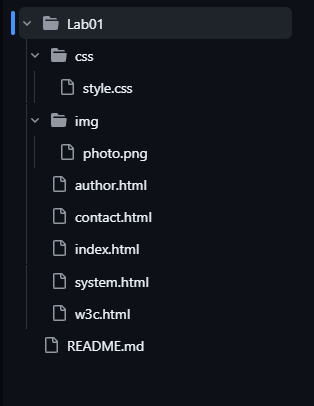
\includegraphics[width=0.9\textwidth]{img/evidencia1.png}
    \caption{Estructura del Laboratorio 01 en GitHub.}
\end{figure}
% ------------------------------------------------------------
\subsection{Historial de commits}

La siguiente evidencia debe mostrar los commits realizados
durante el desarrollo del laboratorio.

 \begin{figure}[H]
    \centering
     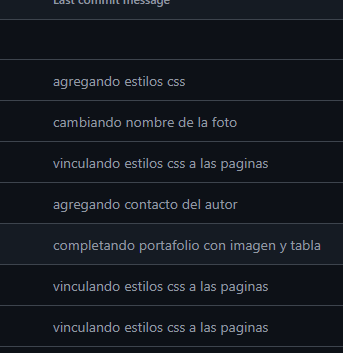
\includegraphics[width=0.9\textwidth]
     {img/evidencia2.png}
    \caption{Historial de commits del Laboratorio 01.}
 \end{figure}

% ------------------------------------------------------------
\subsection{Herramientas de desarrollador}

Se debe incluir una captura de la pestaña Network del navegador,
donde se pueda observar una solicitud HTTP y su código de estado.

 \begin{figure}[H]
     \centering
    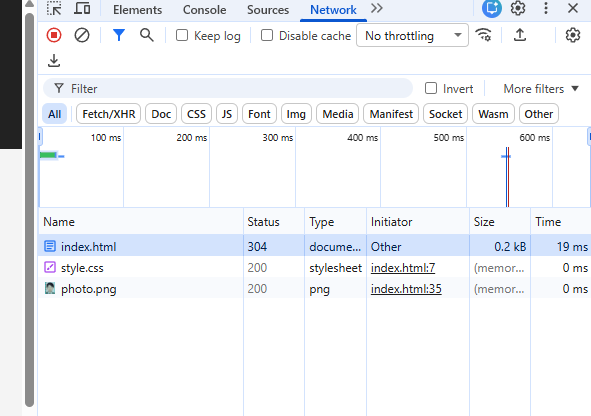
\includegraphics[width=0.9\textwidth]
     {img/evidencia3.png}
     \caption{Solicitud HTTP observada mediante DevTools.}
 \end{figure}

% ------------------------------------------------------------
\subsection{Página web publicada}

Se debe incluir una captura de la página publicada mediante
GitHub Pages.

 \begin{figure}[H]
     \centering
    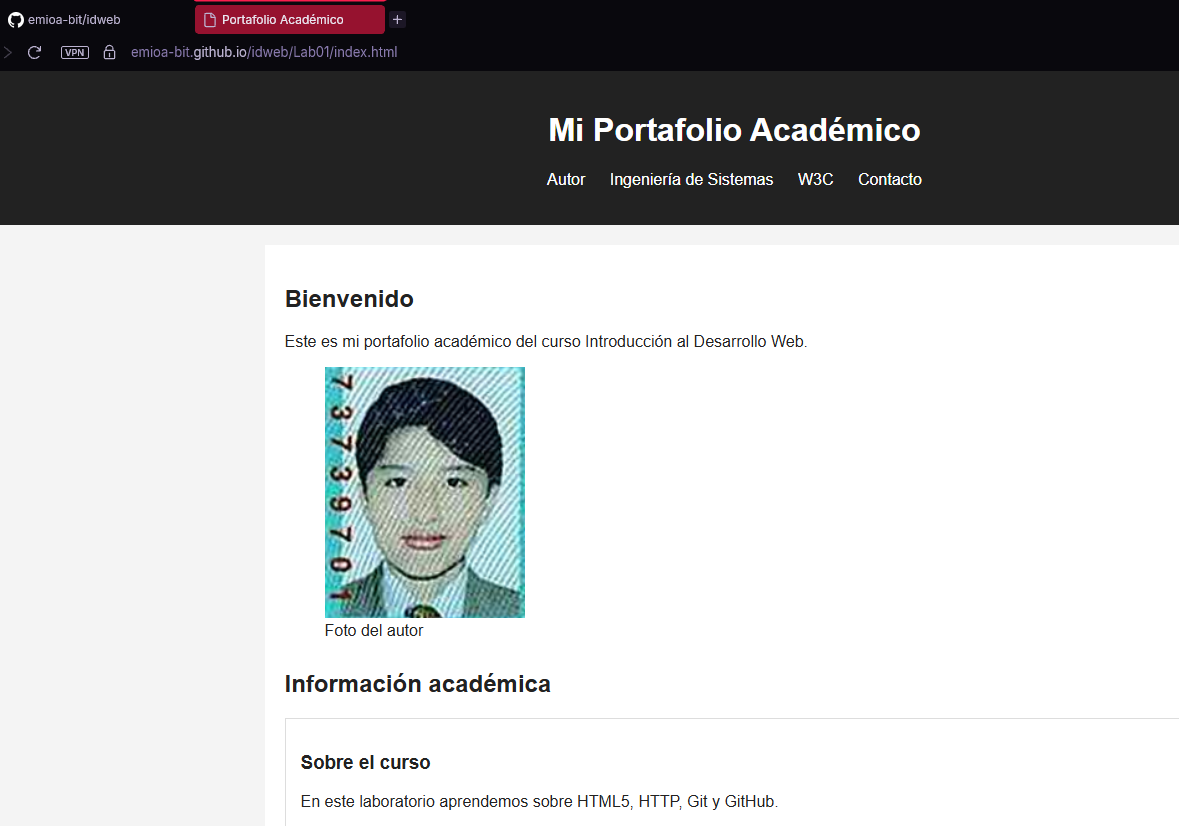
\includegraphics[width=0.9\textwidth]
    {img/evidencia4.png}
    \caption{Portafolio académico publicado mediante GitHub Pages.}
\end{figure}

% ============================================================
% CUESTIONARIO
% ============================================================

\section{Cuestionario}

% ------------------------------------------------------------
\subsection{1. ¿Qué significan los códigos HTTP 200, 301,
404 y 500?}

\begin{itemize}

    \item \textbf{200}: la solicitud fue procesada correctamente.

    \item \textbf{301}: el recurso fue trasladado permanentemente.

    \item \textbf{404}: el recurso solicitado no fue encontrado.

    \item \textbf{500}: ocurrió un error interno en el servidor.

\end{itemize}

% ------------------------------------------------------------
\subsection{2. ¿Cuál es la diferencia entre HTML semántico
y utilizar solamente elementos div?}

HTML semántico utiliza elementos que describen el significado
y función del contenido, como \texttt{header}, \texttt{nav},
\texttt{main}, \texttt{section}, \texttt{article} y
\texttt{footer}.

El uso excesivo de elementos \texttt{div} no proporciona
información semántica sobre el contenido.

El HTML semántico facilita la accesibilidad, la organización
del documento y la interpretación del contenido por parte de
los motores de búsqueda.

% ------------------------------------------------------------
\subsection{3. ¿Qué importancia tiene la etiqueta viewport?}

La etiqueta viewport permite controlar la forma en que una
página se adapta a diferentes tamaños de pantalla.

Se utiliza mediante:

\begin{lstlisting}[language=HTML]
<meta name="viewport"
      content="width=device-width, initial-scale=1.0">
\end{lstlisting}

Esta configuración es importante para desarrollar páginas
adaptables a dispositivos móviles.

% ------------------------------------------------------------
\subsection{4. ¿Qué diferencia existe entre Git y GitHub?}

Git es un sistema distribuido de control de versiones que
permite registrar cambios realizados en un proyecto.

GitHub es una plataforma que permite almacenar repositorios
Git de manera remota y colaborar con otras personas.

% ------------------------------------------------------------
\subsection{5. ¿Cuál es la función de git add, git commit
y git push?}

\begin{itemize}

    \item \textbf{git add}: prepara los archivos modificados
    para ser incluidos en un commit.

    \item \textbf{git commit}: registra los cambios en el
    historial local del repositorio.

    \item \textbf{git push}: envía los commits del repositorio
    local hacia el repositorio remoto.

\end{itemize}

% ------------------------------------------------------------
\subsection{6. ¿Por qué es importante mantener un historial
de commits?}

El historial de commits permite conocer la evolución del proyecto,
identificar los cambios realizados y recuperar versiones
anteriores cuando sea necesario.

También permite al profesor revisar el proceso de desarrollo
del laboratorio.

% ------------------------------------------------------------
\subsection{7. ¿Cuál es la ventaja de organizar los laboratorios
en carpetas como Lab01 y Lab02?}

La organización mediante carpetas permite separar los archivos
correspondientes a cada laboratorio.

Esto facilita la revisión del repositorio y evita mezclar
archivos de diferentes actividades.

% ------------------------------------------------------------
\subsection{8. ¿Qué puede revisar el profesor en GitHub?}

El profesor puede revisar el código fuente, la estructura del
proyecto, los commits realizados, las fechas de modificación,
los archivos HTML y CSS, y las páginas publicadas.

También puede comprobar la evolución del trabajo mediante
el historial del repositorio.

% ============================================================
% CONCLUSIONES
% ============================================================

\section{Conclusiones}

\begin{itemize}

    \item Se aprendió a utilizar una estructura HTML5 semántica
    para organizar correctamente una página web.

    \item Se comprendió la función básica del protocolo HTTP
    y sus principales códigos de respuesta.

    \item Se utilizaron las herramientas de desarrollador
    del navegador para observar solicitudes HTTP.

    \item Se implementaron elementos orientados a la
    accesibilidad, como atributos \texttt{alt}, etiquetas
    \texttt{label} y encabezados estructurados.

    \item Se aprendió a organizar un proyecto web mediante
    carpetas y archivos HTML y CSS.

    \item Se utilizó Git y GitHub para registrar y almacenar
    los avances del laboratorio.

    \item GitHub Pages permitió publicar el proyecto y comprobar
    el funcionamiento de las páginas desarrolladas.

\end{itemize}

% ============================================================
% ESTRUCTURA FINAL
% ============================================================

\section{Estructura final del Laboratorio 01}

La estructura final del proyecto es:

\begin{lstlisting}[style=ascii-tree]
IDWeb/
|--- Lab01/
|   |--- index.html
|   |--- author.html
|   |--- system.html
|   |--- w3c.html
|   |--- contact.html
|   |
|   |--- css/
|   |   |--- style.css
|   |
|   |--- img/
|       |--- photo.png
|       |--- evidencia_estructura.png
|       |--- evidencia_commits.png
|       |--- evidencia_http.png
|       |--- evidencia_pages.png
\end{lstlisting}

% ============================================================
% RÚBRICA
% ============================================================

\section{\textcolor{red}{Rúbricas}}

\subsection{\textcolor{red}{Entregable Informe}}

\begin{table}[H]

\caption{Tipo de Informe}

\setlength{\tabcolsep}{0.5em}

{\renewcommand{\arraystretch}{1.5}

\begin{tabular}{|p{3cm}|p{12cm}|}

\hline

\multicolumn{2}{|c|}{\textbf{\textcolor{red}{Informe}}}

\\
\hline

\textbf{\textcolor{red}{Latex}}
&
\textcolor{blue}{
El informe está en formato PDF generado mediante
LaTeX, con una presentación ordenada y fácil de leer.
}

\\
\hline

\end{tabular}

}

\end{table}

% ============================================================
% NIVELES DE DESEMPEÑO
% ============================================================

\subsection{\textcolor{red}{Rúbrica para el contenido del Informe}}

\begin{itemize}

    \item Se marcará la columna Checklist de acuerdo con los
    criterios cumplidos.

    \item El estudiante realizará una autocalificación de acuerdo
    con los niveles de desempeño.

\end{itemize}

\begin{table}[H]

\caption{Niveles de desempeño}

\begin{center}

\begin{tabular}{ccccc}

\hline

&
\multicolumn{4}{c}{Nivel}

\\

\cline{1-5}

\textbf{Puntos}
&
Insatisfactorio 25\%
&
En Proceso 50\%
&
Satisfactorio 75\%
&
Sobresaliente 100\%

\\

\hline

\textbf{2.0}
&
0.5
&
1.0
&
1.5
&
2.0

\\

\textbf{4.0}
&
1.0
&
2.0
&
3.0
&
4.0

\\

\hline

\end{tabular}

\end{center}

\end{table}

% ============================================================
% RÚBRICA FINAL
% ============================================================

\begin{table}[H]

\caption{Rúbrica para contenido del Informe y demostración}

\setlength{\tabcolsep}{0.5em}

{\renewcommand{\arraystretch}{1.5}

\begin{tabular}{|p{2.7cm}|p{7cm}|x{1.3cm}|p{1.2cm}|p{1.5cm}|p{1.1cm}|}

\hline

\multicolumn{2}{|c|}{Contenido y demostración}
&
Puntos
&
Checklist
&
Estudiante
&
Profesor

\\
\hline

\textbf{1. GitHub}
&
Hay enlace URL activo del directorio para el laboratorio
hacia su repositorio GitHub con código fuente terminado y
fácil de revisar.
&
2
&
X
&
2
&
\\

\hline

\textbf{2. Commits}
&
Hay capturas de pantalla de los commits más importantes
con sus explicaciones detalladas.
&
4
&
X
&
1
&
\\

\hline

\textbf{3. Código fuente}
&
Hay porciones de código fuente importantes con numeración
y explicaciones detalladas de sus funciones.
&
2
&
X
&
1
&
\\

\hline

\textbf{4. Ejecución}
&
Se incluyen ejecuciones y pruebas del proyecto explicadas
gradualmente.
&
2
&
X
&
1
&
\\

\hline

\textbf{5. Pregunta}
&
Se responde con completitud a las preguntas formuladas
en la tarea.
&
2
&
X
&
2
&
\\

\hline

\textbf{6. Fechas}
&
Las fechas de modificación del código fuente están dentro
de los plazos establecidos.
&
2
&
X
&
2
&
\\

\hline

\textbf{7. Ortografía}
&
El documento no presenta errores ortográficos.
&
2
&
X
&
2
&
\\

\hline

\textbf{8. Madurez}
&
El informe muestra la evolución del proyecto, explicaciones
precisas y una presentación adecuada.
&
4
&
X
&
1
&
\\

\hline

\multicolumn{2}{|c|}{\textbf{Total}}
&
20
&
&
12
&

\\

\hline

\end{tabular}

}

\end{table}

% ============================================================
% REFERENCIAS
% ============================================================

\clearpage

\section{Referencias}

\begin{itemize}

    \item World Wide Web Consortium (W3C).
    \url{https://www.w3.org/}

    \item MDN Web Docs.
    \url{https://developer.mozilla.org/}

    \item GitHub.
    \url{https://github.com/}

    \item HTML Living Standard.
    \url{https://html.spec.whatwg.org/}

\end{itemize}

% ============================================================

\end{document}